\documentclass{standalone}
\usepackage{tikz}
\usepackage{ctex,siunitx}
\setCJKmainfont{Noto Serif CJK SC}
\usepackage{tkz-euclide}
\usepackage{amsmath}
\usetikzlibrary{patterns, calc}
\usetikzlibrary {decorations.pathmorphing, decorations.pathreplacing, decorations.shapes,}
\begin{document}
\small
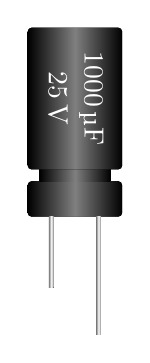
\begin{tikzpicture}[>=stealth,scale=3.0]
  \fill[left color=black,right color=black,middle color=gray,rounded corners=0.5mm]
  (-0.2,0)rectangle(0.2,0.15);
  \fill[left color=black,right color=black,middle color=gray](-0.15,0.15)rectangle(0.15,0.3);
  \fill[left color=black,right color=black,middle color=gray,rounded corners=0.5mm](-0.2,0.20)rectangle(0.2,0.8);
  \fill[left color=gray,right color=gray,middle color=white](-0.11,0)rectangle(-0.09,-0.3);
  \fill[left color=gray,right color=gray,middle color=white](0.11,0)rectangle(0.09,-0.5);
  \node at (0.07,0.5)[text=white,rotate=-90]{\qty{1000}{\micro F}};
  \node at (-0.07,0.5)[text=white,rotate=-90]{\qty{25}{V}};
\end{tikzpicture}
\end{document}